%!TEX root = ../../Heun_Dale_Haney_A_dynamic_approach_to_input_output_modeling.tex
%%%%%%%%%%%%%%%%%%%%% chapter.tex %%%%%%%%%%%%%%%%%%%%%%%%%%%%%%%%%
%
% sample chapter
%
% Use this file as a template for your own input.
%
%%%%%%%%%%%%%%%%%%%%%%%% Springer-Verlag %%%%%%%%%%%%%%%%%%%%%%%%%%
%\motto{Use the template \emph{chapter.tex} to style the various elements of your chapter content.}

%%%%%%%%%%%%%%%%%%%%%%%%%%%%%%%%%%%%%%%%%%%%%%%%%%%%%%%
%%%%%%%%%% Conceptual and Theoretical Isseus %%%%%%%%%%
%%%%%%%%%%%%%%%%%%%%%%%%%%%%%%%%%%%%%%%%%%%%%%%%%%%%%%%
\chapter{Unfinished Business: Practical, Methodological, and Theoretical Issues}
% Always give a unique label
\label{chap:unfinished_business}
% use \chaptermark{} to alter or adjust the chapter heading in the running head
\chaptermark{Issues}
%%%%%%%%%%%%%%%%%%%%%%%%%%%%%%%%%%
%%%%%%%%%%%%%%%%%%%%%%%%%%%%%%%%%%
%%%%%%%%%%%%%%%%%%%%%%%%%%%%%%%%%%

\abstract*{[NEED TO ADD ABSTRACT HERE]}

%% \abstract{Each chapter should be preceded by an abstract (10--15 lines long) that summarizes the content. The abstract will appear \textit{online} at \url{www.SpringerLink.com} and be available with unrestricted access. This allows unregistered users to read the abstract as a teaser for the complete chapter. As a general rule the abstracts will not appear in the printed version of your book unless it is the style of your particular book or that of the series to which your book belongs.\newline\indent
%% Please use the 'starred' version of the new Springer \texttt{abstract} command for typesetting the text of the online abstracts (cf. source file of this chapter template \texttt{abstract}) and include them with the source files of your manuscript. Use the plain \texttt{abstract} command if the abstract is also to appear in the printed version of the book.}

%% Use the template \emph{chapter.tex} together with the Springer document class SVMono (monograph-type books) or SVMult (edited books) to style the various elements of your chapter content in the Springer layout.


With any endeavor of this magnitude, 
namely development and comprehensive presentation 
of a framework for economies of the world,
unfinished business is inevitable. 
This chapter discusses several 
practical, methodological, and theoretical issues
that should be addressed in the future.
On a practical level, additional data are needed 
to fully utilize the framework developed herein.
In terms of methodological issues, we encourage that economists of all types
embrace material, energy, embodied energy, and economic value counting 
as a valid method of inquiry for modern economics.
And, there are issues of co-products and the choice of the energy input vector
that need to be addressed.  
Finally, several theoretical issues, including
material and energy quality, 
model boundaries, and 
the Sun
are addressed.
We begin with the topic of data.


%%%%%%%%%% Metabolic Economy Models %%%%%%%%%%
\section{Metaphors and models}
\label{sec:metaphors_and_models}
%%%%%%%%%%

**** Mik: Consider moving this section or a version of this section 
to the introduction when you get back to reviewing the introduction. ****

**** If move to introduction, be sure to refer to it in the Conclusion. ****

**** Becky: Add a paragraph about economic metaphors here. ****

Historically, mainstream economists have used the metaphor of \emph{machine}
to describe economies. 
In fact, much of mathematical economic modeling today 
relies upon mechanistic conceptual foundations whose roots 
are in Newtonian physics\index{Newtonian physics} 
and The Enlightenment\index{Enlightenment, The}.\footnote{The subfield 
of longwave economic growth modeling, in particular, 
uses mechanistic language to describe their equations. 
For example, Jones~\cite[pp. 6 \& 18]{Jones:2001wn} 
refers to the ordinary differential equations 
that describe births, deaths, and the production of ideas
as ``laws of motion.''}
If your metahpor is a machine, it makes sense to analyze economies
with equations that describe machines.
In the mainstream, such equations usually, but not exclusively or restrictively,
are developed assuming that the economic machine is a \emph{closed} system.

In this book, we take the strong position that economies are
better-represented as open, organic metabolisms.
Many ecological economists, 
who are predisposed to view the economy as a metabolism,
reject the use of mechanistic equations 
to describe the economy, in part because such equations often assume a 
machine that operates independently from the biosphere.
Other ecological economists dismiss mainstream economics 
and its mechanistic models out of hand. 
For example, S{\"o}llner pejoratively says 
``The prime example of physics envy and the desire 
to emulate the natural sciences is, of course, 
neoclassical economics which was explicitly and purposefully 
copied from classical mechanics.''~\cite[p. 178]{Sollner:1997wx}

But, it doesn't have to be this way.
We claim that it is not the use of equations 
and mathematical models themselves that is the problem.
Rather, it is the application of such equations 
to an assumed closed system
that is is worthy of criticism.
Thus, our approach herein includes rigorous application of the 
admittedly mechanistic accounting equations 
for materials, energy, embodied energy, and economic value
\emph{under the assumption of} and \emph{including} 
vigorous and necessary interactions between
the economy and the biosphere.

It is our hope that this book will allow

\begin{itemize}
	\item{mainstream economists to see that}
	\begin{itemize}
		\item{the metabolism metaphor is apt because 
		interaction between the economy and the biosphere is 
		what drives economic growth and}
		\item{rigorous mechanistic models can and should include 
		interactions between the biosphere and the economy, and} 
	\end{itemize}
	\item{ecological economists to see that rigorous mathematical modeling
	is an important tool for understanding interactions
	between the economy and the biosphere.}
\end{itemize}

In summary, we encourage both mainstream and ecological economists
to embrace mathematical modeling of 
material, 
energy, 
embodied energy, 
and economic value flows
both within the economy and between the economy and the biosphere
as a valid method of inquiry for modern economics.



%%%%%%%%%% Data %%%%%%%%%%
\section{Subjective vs.\ intrinsic theory of value}
\label{sec:theory of value}
%%%%%%%%%%

As stated in Chapter~\ref{chap:value}, the neoclassical approach 
is a \emph{subjective} theory of value. 
It is determined by the relative ability of the product to satisfy a person’s wants. 
However, a person’s wants are malleable and are, in turn, formed within a 
``constellation of shared goals to which a society aspires.''~\cite{Costanza:2004we}
Thoughout history, economists (particularly the classicals) 
and non-economists have searched for an invariant, objective, 
\emph{intrinsic} determinant of value.\footnote{Following the ecological economics literature, 
we use the term, intrinsic, in the sense of ``objective.'' Costanza~\cite{Costanza:2004we} 
notes that a better term would be objective in order to avoid moral overtones associated 
with the term intrinsic.} 
Adam Smith, Karl Marx, David Ricardo and his student Sraffa all proposed 
alternative determinants of value.  
Their proposed objective values were based on identifying the primary input into production,
such as labor or land and using that input in the sense of a numeraire. 
That is, a way to measure value across the entire spectrum 
of goods and services in commensurate units.

Costanza~\cite{Costanza:2004we} makes a compelling case for energy 
as the only truly primary input into production 
and thus an, or rather the, objective determinant of value. 
On a global scale, he notes, (solar) energy 
(including that which is stored in fossil fuels) is the only primary input into production, 
everything else is an intermediate input. 
Thus, free energy could be seen as not simply an input into production, 
but the primary input into production, upon which an objective (intrinsic), 
energy theory of value could be built. 
In fact, this line of research has yielded some interesting figures on the amount 
of solar energy required to run the economy. 
See Section~\ref{sec:emergy} for further discussion.

We work within the neoclassical framework for pragmatic, rather than philosophical, reasons. 
It is currently not an adequate 
framework for guiding economies situated within a ``full'' earth. For example, 
Herman Daly~\cite{daly1995} provides important discussion 
of the focus on ``value-added.'' % chktex 38
The neoclassical framework focuses on measuring value-added 
and ignores the quality of the resources to which the value is being added. 
This leads to overstatement of economic value flows in the following way. 
As easily accessible forms of energy (e.g.,  oil extracted from the Texas panhandle) 
are used up and more difficult locations must be tapped (e.g., Alaskan north slope) 
the economy appears to grow.
The ``value-added'' by human and manufactured capital is higher, 
the more work humans must do to extract domestic energy sources. 
However, what is actually happening is that the stock  of  natural resource is diminishing. 
Or, stated differently, the subsidy that nature provides the economy is declining.

Therefore, as ``that to which value is added'' diminishes, 
economic growth begins to reach binding constraints.
Daly, Costanza and others ****include other references here**** discuss the importance of 
identifying the economic scale---amount of materials put through the economy---that 
is viable for the biosphere to handle. 
The neoclassical framework is not able to address this larger question without modification.

While we do not attempt to correct this widely utilized approach, 
we note that our model provides a natural starting place for extending the neoclassical framework. 
Value flows to and from the biosphere can be estimated and included in the model, 
once a system of envrionmental-economic accounting is in place. 
Eventually, the framework will reconnect the economy to the biosphere 
as in Figure~\ref{fig:basic_value_with_biosphere_flows}.\footnote{As of this printing, 
the System of Environmental-Economic Accounting (SEEA)~\cite{UNSEEA:aa}
is in its third revision 
using a process of global consultation. 
This system contains internationally agreed-upon standards for quantifying value flows 
to and from the biosphere. 
This is a system analogous to the System of National Accounts (SNA) 
produced by the same United Nations organization
which is a framework for measuring economic value creation consistently across nations.}

%**** MIK---can you create a fig. 5.3? Add in 0j and j0 value flows as dashed lines? 
%(I referred to it with label  basic\_value\_with\_biosphere\_flows) ****

\begin{figure}[h!]
\centering\
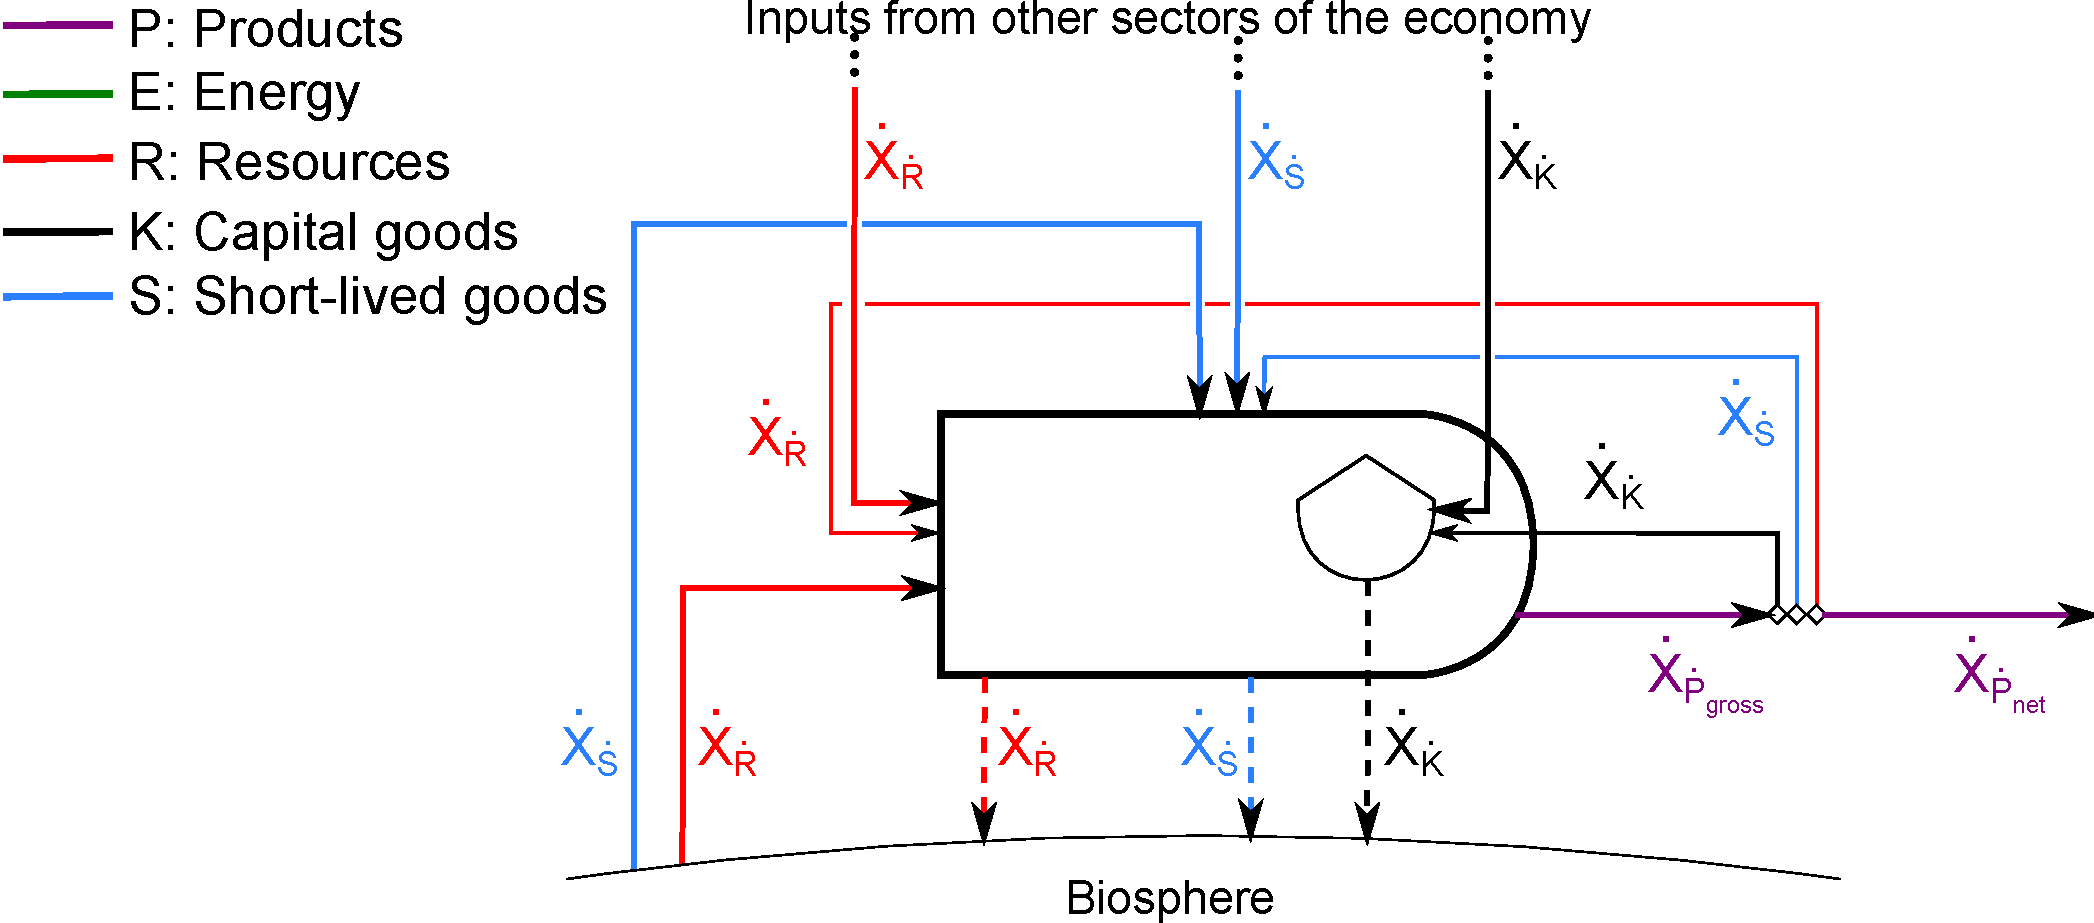
\includegraphics[width=0.8\linewidth]{Part_3/Chapter_Unfinished/images/PERKS_basic_unit_value_with_biosphere_flows.pdf}
\caption[Aggregated flows of value for a single sector including flows to and from the biosphere]{Aggregated flows of value for a single sector including flows to and from the biosphere.}
\label{fig:basic_value_with_biosphere_flows}
\end{figure}


%%%%%%%%%% Data %%%%%%%%%%
\section{Data}
\label{sec:Data}
%%%%%%%%%%

In Chapter~\ref{chap:intro}, 
we noted the importance of ``counting''
materials, energy, and value as they flow through economies.  
Unfortunately, unless data on these flows 
is collected and disseminated routinely, 
such counting is impossible.
At several points in this manuscript,
we have noted the very practical issue of the
need for additional data, information, and analysis.

In Section~\ref{sec:materials_auto},
our attempt to model the physical flows of 
materials through the US auto industry was
severely hampered by the lack of any data on
material flows.
Work to account such flows is starting to be
addressed at the level of economies,
particularly within Europe~\cite{EUROSTAT2011}.
This work needs to continue as well as the
development of sub-economy,
inter-industry material accounts.
Chapter~\ref{chap:intensity} noted the need to collect
data on human and draught animal physical work input to 
sectors of economies, espeically for those economies where 
muscle work is on the same order of magnitude 
as fossil fuel energy input.

The need for rigorous and accurate data
is all the more pressing in light of the need for
an \emph{independent} method to calculate
the energy intensity of goods and services,
as suggested in Chapter~\ref{chap:intensity}.
If this independent method relies on process-type
analysis,
then there is a critical need for systematic
collection of such data by public agencies
which is currently collected by private organizations.
The latest version of the ecoinvent database (v3)
contains detailed analysis of over 10,000 
processes~\cite{EcoInvent2012}.
This is a fantastic effort, but more needs to be
done to bring this crucial information into the public arena.

Unfortunately, it seems like public agencies are headed in the
opposite direction.
The U.S.\ stopped collecting 
satellite account data\index{satellite account data} in 2000. 
Beyond the U.S., few countries collect and disseminate
the kind of data required as inputs to the framework
developed herein.

The adage ``you can't control what you don't measure''
seems appropriate here. 
As the world confronts significant challenges
of material and energy supplies in the coming years,
it will be impossible to make wise decisions about
which materials to use,
which energy sources to develop, and 
which products to incentivize.

Another adage ``we count what we value and we value what we count''
points out that we are not presently valuing highly enough
the important flows of which our economies are comprised.
We add our voices to those encouraging governments and 
institutions to collect high-quality data on material 
and energy flows.
**** Becky, are there references that call for a renewed focus on 
collecting satellite account data? 
We should point to those references here. ****
 
**** Becky: review the above paragraphs.
Can you provide additional context on the decision
to stop collecting this data? ****

%%%%%%%%%% Hybrid %%%%%%%%%%
\section{Hybrid I-O---process-based methods}
\label{sec:hybrid}
%%%%%%%%%%

In early chapters,
we have made the distinction between
process-based (often called ``bottom-up'') 
and input-output (often called ``top-down'')
analyses.
The advantages and disadvantages of each type
of analysis are outlined in Figure~\ref{fig:IO_vs_process}.

Process analysis is based on detailed technological
or engineering models of specific economic processes.
Model specification and data collection is arduous and
time-consuming.
The aim of the analysis may be to calculate the
energetic and material flows associated with the process
under study by disaggregating the process into
several components or sub-processes.
In reality,
any economic process exists in a complex network of
interacting processes that encompass the entire economy,
as stated by Bullard et al. (1978), 
\begin{quote}
	each step in a process analysis may be viewed as 
	an expansion of the system boundary 
	(around the item being analyzed) 
	into the economic system~\cite[p.281]{Bullard:1978vd}
\end{quote}
and represented diagramatically in Figure~\ref{fig:Hybrid_boundary}.
Every process calls on every other process within the economy,
even if only minutely and indirectly at many steps removed.
Obviously,
the time, 
effort and cost involved with trying to model and
measure all of the flows involved become daunting
for even low numbers of interacting processes.
The decision of where to draw the boundary of
a process analysis is known in the 
lifecycle assessment literature as the 
\emph{truncation problem}~\cite{Suh2004}.
One method to extend the comprehensiveness of process
analyses is to use a hybrid method,
utilizing data from an I-O analysis to supplement the
missing data from the truncation of the process analysis.
The financial cost of goods and services identified by
the process analysis are converted to energy
(or material) flows via the I-O method.
The truncation error is replaced by a smaller aggregation
error due to limitations of the I-O 
method~\cite{Bullard:1978vd}.
A variety of hybrid methods exist which aim to
overcome the limitations of either method 
individually~\cite{Bullard:1978vd, Suh2004, Suh2002, 
Crawford2008, Zhai2010}


\begin{figure}[h!]
\centering\
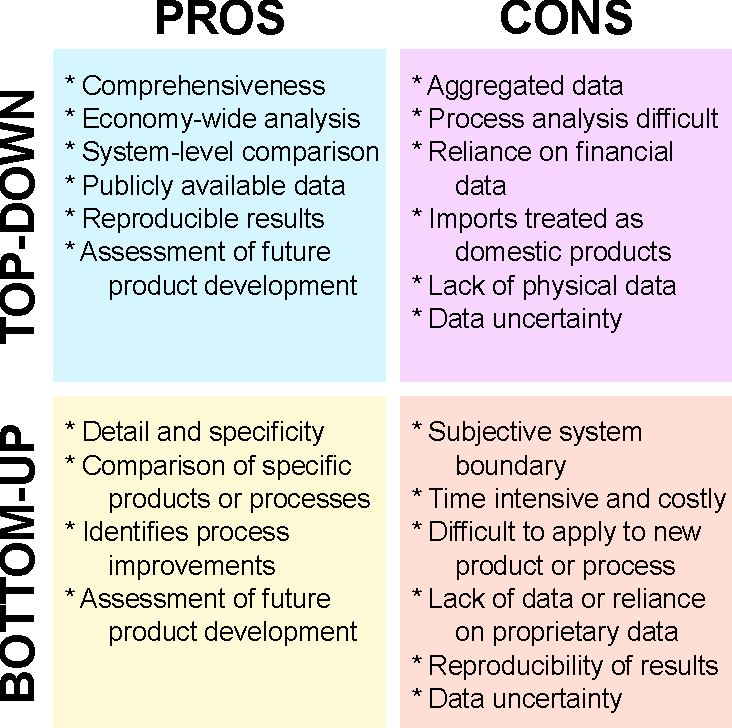
\includegraphics[width=0.8\linewidth]{Part_3/Chapter_Unfinished/images/Top_down_vs_bottom_up.pdf}
\caption[Top-down vs.\ bottom-up analyses ]{Advantages (pros) and disadvantages (cons) of ``top-down'', I-O and ``bottom-up'', process-based analyses, adapted from \cite{Hendrickson2006}.}
\label{fig:IO_vs_process}
\end{figure}

\begin{figure}[h!]
\centering\
\includegraphics[width=\linewidth]{Part_3/Chapter_Unfinished/images/Hybrid_boundary.pdf}
\caption[System boundary for process and I-O analyses]{System boundary for process and I-O analyses, adapted from \cite{Bullard:1978vd}.}
\label{fig:Hybrid_boundary}
\end{figure}


%%%%%%%%%% Second Law %%%%%%%%%%
\section{Resource quality and irreversibility}
\label{sec:resource_quality_and_irreversibility}
%%%%%%%%%%

The quality of both materials\index{materials!quality of} 
and energy\index{energy!quality of} play a role in the 
efficiency with which economies use energy resources to convert material resources into products.
The following two sections briefly discuss both.
Thereafter, we raise the issue of thermodynamic 
irreversibility\index{thermodynamic irreversibility}\index{irreversibility!thermodynamic|see{thermodynamic irreversibility}}.

%+++++++++ Material Quality ++++++++++
\subsection{Quality of materials}
\label{sec:material_quality}
%+++++++++

% **** Mik: Please review and add to this draft section. --Matt ****

The concept of material quality has connections to our framework in two ways:
\begin{enumerate}
	\item 
		first is Georgescu-Roegen's so-called ``Fourth Law of
		Thermodynamics'';
	\item		
		second is (decline of) the quality of 
		natural resources	within the biosphere.
\end{enumerate}

Georgescu-Roegen proposed a 
Fourth Law of Thermodynamics\index{Fourth Law of Thermodynamics}\index{Thermodynamics!Fourth Law|see{Fourth Law of Thermodynamics}}
which states that ``In a closed system, 
the material entropy must ultimately reach a maximum:'' 
material degrades, just as energy.\cite{GeorgescuRoegen:1977tf}
For example, consumption of coal to produce electricity
results in CO$_2$ and ash that cannot
be reprocessed into coal.
Although mass (measured in kilograms) is conserved through processes, 
CO$_2$ and ash are significantly less useful than coal,
and Georgescu-Roegen claims that we need a way to account
for the loss of material quality.

Furthermore, initial extraction of easy-to-reach ores 
and fossil fuel resources (coal and oil)
leads, over time, to a reduction in the quality 
of material resources (ore grades decrease over time) 
**** Mik: do you have a reference for this? ****
and increased energy resources needed to perform extraction.


%+++++++++ Energy Quality ++++++++++
\subsection{Quality of energy}
\label{sec:energy_quality}
%+++++++++

There are several ways to assess the quality of energy.
The Second Law of Thermodynamics provides, among other things,
a framework for discussing the \emph{quality} of energy.
Hammond and Winnett~\cite{Hammond:2009tu} reviewed
the influence of thermodynamics on ecological economics 
and noted the importance of the concept of \emph{exergy},
which combines the First and Second Laws of thermodynamics
to describe the maximum physical work obtainable from an energy source:

\begin{quote}
	[i]n a sense [exergy] represents the thermodynamic `quality' 
	of an energy carrier, 
	and that of the waste heat or energy lost in the reject stream. 
	Electricity, for instance, may be regarded as an energy carrier having a high quality, 
	or exergy, because it can undertake work. 
	In contrast, low temperature hot water, although also an energy source, 
	can only be used for heating purposes. 
	This distinction between energy (strictly enthalpy) and exergy is very important 
	when considering a switch, for example, 
	from traditional internal combustion engines to electric, hybrid, or fuel cell vehicles. 
	Thus, \ldots{} it is important to employ exergy analysis 
	alongside a traditional First Law energy analysis in order to illuminate these issues.
\end{quote}

The quality of energy can be assessed in terms of its economic value, too.
Some energy sources have been shown to be more economically valuable in their use
than others.
And, ``accounting for energy quality reveals a relatively strong relationship 
between energy use and economic output.''~\cite[p. 313]{Cleveland2000}


%+++++++++ Irreversibility ++++++++++
\subsection{Process irreversibility}
\label{sec:irreversibility}
%+++++++++

Irreversibility is the concept that naturally-occurring processes 
are uni-directional.
For example, the flow of electrical current through a resistor
generates heat;
however, pointing an operating hairdryer at an electrical resistor 
does \emph{not} produce electricity.
Considering the production of electricity from coal,
we note that both important processes within a power plant are \emph{irreversible}:

\begin{itemize}
	\item{the combustion process that converts coal to CO$_{2}$ and ash 
	(with associated thermal energy release, $\dot{Q}$) and}
	\item{the heat transfer process wherein $\dot{Q}$ flows 
	from high temperature to low temperature (with associated mechanical work production).}
\end{itemize}

\noindent{}Thermal energy does not naturally flow from low temperature to high temperature.
And, ash and CO$_{2}$ do not naturally combine to form coal.

The concepts of resource quality and irreversibility are linked.
One statement of the Second Law indicates that heat flow is irreversible: 
it goes from hot to cold only. 
Because lower-temperature heat is less useful, 
we say that the thermal energy has degraded when it used (becomes colder).
The proposed Fourth Law is similar: 
materials are degraded through their use.
Georgescu-Roegen's proposed Fourth Law establishes an analogy between
(a) the Second Law of Thermodynamics,\index{Second Law of Thermodynamics} 
in which energy quality degrades with use and
(b) the Fourth Law of Thermodynamics,\index{Fourth Law of Thermodynamics}
in which material quality degrades with use.\footnote{The analogy 
	between the First and Fourth Laws of Thermodynamics
	are similar to the analogy between 
		(a) the Law of Conservation of Mass\index{conservation of mass}, 
		in which mass can be neither created nor destroyed and 
		(b) the First Law of Thermodynamics\index{First Law of Thermodynamics}, 
		in which energy can be neither created nor destroyed.}

We recommend that future work be done to incorporate 
resource quality and irreversibility isses 
into our framework.


%%%%%%%%%% Make-Use %%%%%%%%%%
\section{Co-products}
\label{sec:make-use}\index{co-products}
%%%%%%%%%%

The intersection between our materials, energy, and value accounting framework 
and the I-O literature has been developed under the assumption 
that each economic sector makes a single product ($\dot{P}$).
In particular, the matrix mathematics of Chapter~\ref{chap:intensity}
relies heavily on this assumption 
from the early days of the I-O method.\cite{Bullard:1978vd}
However, the I-O method has been extended 
in the literature to include
co-products for each economic sector.\cite{Costanza:1984tq,Casler1984} 
To do so, both \emph{make} and \emph{use} data are employed.

We decided to leverage the older,
single-product formulation of the I-O method
for the purposes of simplicity. 
The materials, energy, and value accounting framework
presented herein is more easily understood 
without the complexity of the make-use formulation 
of the I-O method.
However, work remains to adapt the materials and energy framework
developed herein to the make-use formulation of the I-O method.


%%%%%%%%%% People as capital stock %%%%%%%%%%
\section{Are people capital stock?}
\label{sec:people_as_stock}
%%%%%%%%%%

**** Mik: complete this section. ****

There is an open
question as to what sort of \emph{stuff} 
should be included as the capital
that accumulates within society. 
Should the material constituting literal
\emph{human capital}, 
i.e.~human bodies, 
be included. 
If humans are to be included within $K_{1}$, 
the resource needed to produce the necessary capital
flow ($\dot{K}_{11}$) is food. 
Food itself represents a large ``resource''
flow and has a large associated energy content. 
Additionally, 
within industrial economies, 
a large amount of energy resources 
are channeled toward the production of food, 
meaning that the \emph{embodied energy}
of food may actually be several times larger than
the actual energy content of the food itself. 
Further questions arise. 
What is the ``product'' of society? 
A materialistic view might hold that the product of
society is human bodies and the labor they can accomplish. 
If so, 
should the agriculture industry 
be accounted as part of the energy sector 
becuase its aim is to provide 
an energy sevice (labor)? 
For non-industrial, agrarian societies, 
the proportion of total energy flow 
comprised by manual (or draught) energy 
may be large. 
In industrialized societies, 
it may be negligible, 
however, 
the energy flows necessary to support agriculture
may be many times larger than the food energy
(and certainly many times larger 
than the labor energy) 
delivered. 
Agrarian societies
are necessarily constrained by the fact that the energy content of the food delivered 
\emph{must be} greater than the labor (and draught) energy required to produce it.
Another view is that societal capital ($K_{1}$) includes only man-made capital, 
i.e.\ items manufactured by humans,
but not humans themselves. 
For the purposes of the framework outlined in this book, 
we shall favor the latter view.
Other researchers favor the opposing view.\cite{Giampietro2013}
However,
the framework presented is general enough to encompass either point of view.
% **** Refer to Giampietro (who includes stocks of people). ****


%%%%%%%%%% The Sun %%%%%%%%%%
\section{What about the sun?}
\label{sec:emergy}
%%%%%%%%%%

Costanza~\cite{Costanza:1978vd} included an option to consider 
solar energy\index{solar energy} as an input to the economy, 
thereby significantly increasing the energy intensity 
of agricultural sectors and other sectors 
that depend upon agricultural outputs. 
However later work by Costanza~\cite{Costanza:1984tq,Costanza:1980ww} 
did not include solar input to the economy.
Whether solar input to the economy 
should be considered in a materials, energy, and economic value 
accounting framework is probably dependent upon 
the objectives of the analysis. 

The motivation for this particular book is primarily 
the effects of declining energy resource quality
due to fossil fuel depletion on industrialized economies. 
As such, inclusion of solar flows is probably unnecessary. 
However, expanding the framework to include non-industrialized 
or agrarian societies may require accounting for solar energy flows. 

There are a number of means by which solar flows can be accounted. 
Solar energy flows could be accounted as short-term flows ($\dot{S}$)
for agricultural and forestry sectors, 
as well as 
solar thermal\index{solar thermal energy}\index{energy!solar thermal|see{solar thermal energy}}, 
solar photovoltaic\index{photovoltaic}, 
wind\index{wind energy}, 
ocean thermal\index{ocean thermal energy}\index{energy!ocean thermal|see{ocean themal energy}}, 
hydro\index{hydro energy}\index{energy!hydro|see{hydro energy}}, and
biomass\index{biomass energy}\index{energy!biomass|see{biomass energy}}
renewable energy\index{renewable energy}\index{energy!renewable|see{renewable energy}}
production sectors.
Doing so would not account for longer-term storage
of solar energy used to form fossil fuels, 
but fossil fuels are already accounted by the $\dot{E}_{0}$ vector
in the framework presented in this book.

A different approach that fully integrates solar 
into an energy framework is \emph{emergy}\index{emergy} accounting.
The emergy method counts \emph{all} material flows 
in terms of \emph{em}bodied solar en\emph{ergy}.\cite{Odum1975, Odum1996}
The basic unit of measure is 
the \emph{em}joule which is often given in terms 
of flows of solar energy embodied in 
the energy (or material)---the solar emjoule\index{emjoule}---per unit of resource, 
abbreviated to seJ/J for energy resources, 
or seJ/g for materials. 
As such, even fossil fuels, e.g.\ coal, 
extracted from the earth have an embodied energy 
of around 67,000~seJ/J.\cite{Brown2004} 


%%%%%%%%%% Endogenous %%%%%%%%%%
\section{What is endogenous?}
\label{sec:what_is_endogenous}
%%%%%%%%%%

There is debate in the literature about whether government\index{government sector} 
and households\index{household sector} 
(so-called ``final consumption'' Figure~\ref{fig:B_materials}) 
should be endogenous to economic models.
This debate is a discussion about the appropriate boundary
for analysis.
Costanza~\cite{Costanza:1980ww} was the first to endogenize government and households, 
because households provide services to the economy (labor) in exchange for wages 
and government provides services to the economy in exchange for taxes, 
both of which require energy. 
Costanza~\cite{Costanza:1980ww} also demonstrated that 
energy intensity\index{energy intensity} results
are a function of boundary (control volume\index{control volume}) selection. 
By including government and households 
as sectors in the model, 
the variation of energy intensity is significantly reduced 
across all sectors of the economy. 

The key energy intensity equation in this book
(Equation~\ref{eq:epsilon_leontief_depreciation_simplification})
was derived under the assumption that ``final consumption''
is exogenous to energy intensity calculation.
However, Equation~\ref{eq:epsilon_leontief_depreciation_simplification}
could be re-derived to endogenize 
``final consumption.''

The total energy\index{total energy} accounting equation for final consumption (1)
in Figure~\ref{fig:C_total_energy} can be written 
analogously to Equations~\ref{eq:C-Total_Energy_Sec_2-b}
and~\ref{eq:C-Total_Energy_Sec_3-b} as

\begin{equation} \label{eq:C-Total_Energy_Sec_1-unfinished}
	\frac{\mathrm{d}B_{K_{1}}}{\mathrm{d}t}
	= \dot{E}_{01}
	+ \varepsilon_{1} \dot{X}_{11}
	+ \varepsilon_{2} \dot{X}_{21}
	+ \varepsilon_{3} \dot{X}_{31}
	- \varepsilon_{1} \dot{X}_{1}
	- \left( \dot{B}_{\dot{R}_{10}} 
							+ \dot{B}_{\dot{S}_{10}}
							+ \gamma_{K,1} B_{K_{1}}
							\right).
\end{equation}

\noindent{}Furthermore, Equations~\ref{eq:C-Total_Energy_Sec_2-b}
and~\ref{eq:C-Total_Energy_Sec_3-b}
can be rewritten as 

\begin{equation} \label{eq:C-Total_Energy_Sec_2-unfinished}
	\frac{\mathrm{d}B_{K_{2}}}{\mathrm{d}t}
	= \dot{E}_{02}
	+ \varepsilon_{1} \dot{X}_{12}
	+ \varepsilon_{2} \dot{X}_{22}
	+ \varepsilon_{3} \dot{X}_{32}
	- \varepsilon_{2} \dot{X}_{2}
	- \left( \dot{B}_{\dot{R}_{20}} 
							+ \dot{B}_{\dot{S}_{20}}
							+ \gamma_{K,2} B_{K_{2}}
							\right)
\end{equation}

\noindent{}and

\begin{equation} \label{eq:C-Total_Energy_Sec_3-unfinished}
	\frac{\mathrm{d}B_{K_{3}}}{\mathrm{d}t}
	= \dot{E}_{03}
	+ \varepsilon_{1} \dot{X}_{13}
	+ \varepsilon_{2} \dot{X}_{23}
	+ \varepsilon_{3} \dot{X}_{33}
	- \varepsilon_{3} \dot{X}_{3}
	- \left( \dot{B}_{\dot{R}_{30}} 
							+ \dot{B}_{\dot{S}_{30}}
							+ \gamma_{K,3} B_{K_{3}}
							\right).
\end{equation}

\noindent{}Following the derivation of Chapter~\ref{chap:intensity},
we can obtain an updated version 
of Equation~\ref{eq:epsilon_leontief_depreciation_simplification}:

\begin{equation} \label{eq:epsilon_leontief_depreciation_simplification_demand_endogenized}
	\bm{\varepsilon} 
	= {(\vec{I} - \vec{A}^{\mathrm{T}})}^{-1}\hat{\vec{X}}^{-1}
		\left[\vec{E}_{0} 
				- \left. \frac{\mathrm{d}\vec{B}_{K}}{\mathrm{d}t} \right|_{\mathrm{other}}
				- \vec{B}_{waste}
		\right],
\end{equation}

\noindent{}wherein 

\begin{itemize}
	\item{the vectors and matrices of Equations~\ref{eq:B_vec_def}--\ref{eq:gamma_hat_matrix_def}
	and~\ref{eq:A_matrix_def} have been extended to include ``final consumption''~(1) and}
	\item{ ``final consumption'' has been endogenized
	(the $\vec{T}_{1}$ term of Equation~\ref{eq:epsilon_leontief_depreciation_simplification}
	has been subsumed into the 
	${(\vec{I} - \vec{A}^{\mathrm{T}})}^{-1}\hat{\vec{X}}^{-1}$
	term of Equation~\ref{eq:epsilon_leontief_depreciation_simplification_demand_endogenized}).}
\end{itemize}

Future work could estimate energy intensity~($\bm{\varepsilon}$) 
using Equations~\ref{eq:epsilon_leontief_depreciation_simplification}
and~\ref{eq:epsilon_leontief_depreciation_simplification_demand_endogenized}
with updated economic data for a wider range of countries.\footnote{Costanza's
analysis~\cite{Costanza:1980ww} was conducted using U.S.\ data for 1963, 1967, and 1972.}
Doing so could provide further insight on Costanza's result~\cite{Costanza:1980ww}
that endogenizing ``final consumption'' reduces variation 
of energy intensity across all sectors of the economy ($\bm{\varepsilon}$).


%%%%%%%%%% Energy Input Vector %%%%%%%%%%
\section{Choice of energy input vector}
\label{sec:energy_input_vector}
%%%%%%%%%%

%**** Mik: please review this section and provide input
%about whether I hit the right tone here.
%I don't want to be too strident, but I also want to 
%be firm. ****

There is discussion in the literature about the $\vec{E}_{0}$
vector and how it should be applied to the economy.
Costanza and Herendeen~\cite{Costanza:1984tq} counted fossil fuel input 
from the biosphere to the economy
at both 
\begin{enumerate}
	\item 	
		the points where direct energy physically 
		enters the economy from the biosphere, 
		typically energy-producing sectors
		(called the DIRECT method\index{DIRECT method}) and
	\item 
		the points of conversion to useful work, 
		typically all energy \emph{consuming} sectors
		(called the DEC method\index{DEC method}, 
		Direct Energy Conversion
		\index{direct energy!conversion|see{DEC methodological}}).
\end{enumerate}
Costanza and Herendeen justified the Direct Energy Conversion~(DEC) 
approach on both thermodynamic and economic grounds. 
The thermodynamic justification derived from the purpose 
of energy consumption in an economy, 
namely to produce useful work. 
If direct energy flows \emph{through} a sector\index{direct energy!flow-through of}, 
it should not be counted \emph{against} that sector: 
only energy that is converted to useful work \emph{within} 
a sector should be counted against that sector.
The economic justification derives 
from the typical treatment of transportation sectors of the economy.
Costanza and Herendeen note:

\begin{quote}
	The primary energy sectors functions [\emph{sic}] \sout{are}
	like the transportation sectors, 
	which alse~[\emph{sic}] require special treatment in I-O analysis 
	based on the difference between the services they provide 
	and their physical inputs and outputs. 
	If a strictly physical interpretation were applied to the 
	transportation sectors\index{transportation sector}, 
	they would receive almost all goods produced in the whole economy as inputs 
	and redistribute them as output, 
	masking information on transfers of goods between sectors. 
	For this reason, the transportation sectors in I-O analysis 
	are thought of as providing transportation services 
	that are purchased by the producing sector, 
	preserving the connection between the producing and consuming sector 
	but adding a `transportation margin.' 
	For analogous reasons, 
	the primary energy sectors should be thought of as providing a 
	`transportation service' in moving primary energy 
	from nature to the consuming sectors. 
	The DEC energy input vector incorporates this interpretation.\cite[p. 151]{Costanza:1984tq}
\end{quote}

The derivation of the materials, energy, and value framework
presented herein counts energy flows from the biosphere to the economy
at the point of physical inflow to the economy. 
That is, elements of the energy input vector 
($\vec{E}_{0}$) are non-zero only for those sectors 
that receive energy directly from the biosphere. 
So, for example, in Figure~\ref{fig:C_energy} from Example~C, 
$\dot{E}_{03} = 0$ and $\dot{E}_{02} \ge 0$. 
Our approach is equivalent to Costanza's DIRECT method.
We believe that the DIRECT approach is correct and that the DEC method is unwarranted.

Justification for our position comes from the detailed derivation
of the materials, energy, and value framework presented in 
Chapters~\ref{chap:materials}--\ref{chap:value}. 

\begin{enumerate}
	\item 
		Firstly, $\vec{E}_{0}$ was defined as a flow 
		from the biosphere to economic sectors
		into which the energy \emph{physically} flows.
		It is inappropriate to route the energy elsewhere.
	\item 
		Secondly, Costanza and Herendeen's 
		concern~\cite[pp. 130 \& 138]{Costanza:1984tq}
		about flow-through of direct energy is unfounded, 
		because direct energy outflows from a sector
		are \emph{never} counted against the sector
		with the DIRECT method.
		We see this fact in the following terms:
			\begin{enumerate}
				\item
					{$- \dot{E}_{1}$ in 
					Equation~\ref{eq:A_total_energy_1},}
				\item
					{$- \dot{E}_{j}$ in Equation~\ref{eq:C-CV_dB_123},}
				\item
					{$- 
						\begin{bmatrix}
							\dot{X}_{2} & 0          \\
							0           & \dot{X}_{3}
						\end{bmatrix}
						\begin{Bmatrix}
							\varepsilon_{2}\\
							\varepsilon_{3}
						\end{Bmatrix}
					$
					in Equation~\ref{eq:C-Expanded_Matrix_Form}, and}
				\item
					{$- \hat{\vec{X}}\bm{\varepsilon}$ 
					in Equation~\ref{eq:matrix_leontief_pre_1}.}
			\end{enumerate}
	\item
		Thirdly, further proof that the DEC approach is unwarranted
		comes from equations that show waste 
		heat~($\dot{Q}_{j0}$) as counting toward 
		the accumulation of embodied energy within 
		an economic sector.
		Equation~\ref{eq:A_dB1/dt} of 
		Section~\ref{subsec:A_first_law_embodied}
		is an example. 
		It is the waste heat~($\dot{Q}_{10}$), 
		i.e.\ the energy \emph{burned within} the sector,
		that counts against the sector.
\end{enumerate}
The DIRECT approach \emph{already always} provides 
the effect that Costanza and Herendeen~\cite{Costanza:1984tq}
desired from the DEC approach. 
Because the DEC approach is unwarranted, 
we quoted DIRECT energy intensity values only
when discussing energy intensities in 
Section~\ref{sec:intensity_auto}.


\bibliographystyle{unsrt}
\bibliography{../../EROI_review_v2}


% Always give a unique label
% and use \ref{<label>} for cross-references
% and \cite{<label>} for bibliographic references
% use \sectionmark{}
% to alter or adjust the section heading in the running head
%% Instead of simply listing headings of different levels we recommend to let every heading be followed by at least a short passage of text. Furtheron please use the \LaTeX\ automatism for all your cross-references and citations.

%% Please note that the first line of text that follows a heading is not indented, whereas the first lines of all subsequent paragraphs are.

%% Use the standard \verb|equation| environment to typeset your equations, e.g.
%
%% \begin{equation}
%% a \times b = c\;,
%% \end{equation}
%
%% however, for multiline equations we recommend to use the \verb|eqnarray|
%% environment\footnote{In physics texts please activate the class option \texttt{vecphys} to depict your vectors in \textbf{\itshape boldface-italic} type - as is customary for a wide range of physical subjects.}.
%% \begin{eqnarray}
%% a \times b = c \nonumber\\
%% \vec{a} \cdot \vec{b}=\vec{c}
%% \label{eq:01}
%% \end{eqnarray}

%% \subsection{Subsection Heading}
%% \label{subsec:2}
%% Instead of simply listing headings of different levels we recommend to let every heading be followed by at least a short passage of text. Furtheron please use the \LaTeX\ automatism for all your cross-references\index{cross-references} and citations\index{citations} as has already been described in Sect.~\ref{sec:2}.

%% \begin{quotation}
%% Please do not use quotation marks when quoting texts! Simply use the \verb|quotation| environment -- it will automatically render Springer's preferred layout.
%% \end{quotation}


%% \subsubsection{Subsubsection Heading}
%% Instead of simply listing headings of different levels we recommend to let every heading be followed by at least a short passage of text. Furtheron please use the \LaTeX\ automatism for all your cross-references and citations as has already been described in Sect.~\ref{subsec:2}, see also Fig.~\ref{fig:1}\footnote{If you copy text passages, figures, or tables from other works, you must obtain \textit{permission} from the copyright holder (usually the original publisher). Please enclose the signed permission with the manucript. The sources\index{permission to print} must be acknowledged either in the captions, as footnotes or in a separate section of the book.}

%% Please note that the first line of text that follows a heading is not indented, whereas the first lines of all subsequent paragraphs are.

% For figures use
%
%% \begin{figure}[b]
%% \sidecaption
% Use the relevant command for your figure-insertion program
% to insert the figure file.
% For example, with the option graphics use
%% \includegraphics[scale=.65]{figure}
%
% If not, use
%\picplace{5cm}{2cm} % Give the correct figure height and width in cm
%
%% \caption{If the width of the figure is less than 7.8 cm use the \texttt{sidecapion} command to flush the caption on the left side of the page. If the figure is positioned at the top of the page, align the sidecaption with the top of the figure -- to achieve this you simply need to use the optional argument \texttt{[t]} with the \texttt{sidecaption} command}
%% \label{fig:1}       % Give a unique label
%% \end{figure}


%% \paragraph{Paragraph Heading} %
%% Instead of simply listing headings of different levels we recommend to let every heading be followed by at least a short passage of text. Furtheron please use the \LaTeX\ automatism for all your cross-references and citations as has already been described in Sect.~\ref{sec:2}.

%% Please note that the first line of text that follows a heading is not indented, whereas the first lines of all subsequent paragraphs are.

%% For typesetting numbered lists we recommend to use the \verb|enumerate| environment -- it will automatically render Springer's preferred layout.

%% \begin{enumerate}
%% \item{Livelihood and survival mobility are oftentimes coutcomes of uneven socioeconomic development.}
%% \begin{enumerate}
%% \item{Livelihood and survival mobility are oftentimes coutcomes of uneven socioeconomic development.}
%% \item{Livelihood and survival mobility are oftentimes coutcomes of uneven socioeconomic development.}
%% \end{enumerate}
%% \item{Livelihood and survival mobility are oftentimes coutcomes of uneven socioeconomic development.}
%% \end{enumerate}


%% \subparagraph{Subparagraph Heading} In order to avoid simply listing headings of different levels we recommend to let every heading be followed by at least a short passage of text. Use the \LaTeX\ automatism for all your cross-references and citations as has already been described in Sect.~\ref{sec:2}, see also Fig.~\ref{fig:2}.

%% Please note that the first line of text that follows a heading is not indented, whereas the first lines of all subsequent paragraphs are.

%% For unnumbered list we recommend to use the \verb|itemize| environment -- it will automatically render Springer's preferred layout.

%% \begin{itemize}
%% \item{Livelihood and survival mobility are oftentimes coutcomes of uneven socioeconomic development, cf. Table~\ref{tab:1}.}
%% \begin{itemize}
%% \item{Livelihood and survival mobility are oftentimes coutcomes of uneven socioeconomic development.}
%% \item{Livelihood and survival mobility are oftentimes coutcomes of uneven socioeconomic development.}
%% \end{itemize}
%% \item{Livelihood and survival mobility are oftentimes coutcomes of uneven socioeconomic development.}
%% \end{itemize}

%% \begin{figure}[t]
%% \sidecaption[t]
% Use the relevant command for your figure-insertion program
% to insert the figure file.
% For example, with the option graphics use
%% \includegraphics[scale=.65]{figure}
%
% If not, use
%\picplace{5cm}{2cm} % Give the correct figure height and width in cm
%
%% \caption{Please write your figure caption here}
%% \label{fig:2}       % Give a unique label
%% \end{figure}

%% \runinhead{Run-in Heading Boldface Version} Use the \LaTeX\ automatism for all your cross-references and citations as has already been described in Sect.~\ref{sec:2}.

%% \subruninhead{Run-in Heading Italic Version} Use the \LaTeX\ automatism for all your cross-refer\-ences and citations as has already been described in Sect.~\ref{sec:2}\index{paragraph}.
% Use the \index{} command to code your index words
%
% For tables use
%
%% \begin{table}
%% \caption{Please write your table caption here}
%% \label{tab:1}       % Give a unique label
%
% For LaTeX tables use
%
%% \begin{tabular}{p{2cm}p{2.4cm}p{2cm}p{4.9cm}}
%% \hline\noalign{\smallskip}
%% Classes & Subclass & Length & Action Mechanism  \\
%% \noalign{\smallskip}\svhline\noalign{\smallskip}
%% Translation & mRNA$^a$  & 22 (19--25) & Translation repression, mRNA cleavage\\
%% Translation & mRNA cleavage & 21 & mRNA cleavage\\
%% Translation & mRNA  & 21--22 & mRNA cleavage\\
%%Translation & mRNA  & 24--26 & Histone and DNA Modification\\
%%\noalign{\smallskip}\hline\noalign{\smallskip}
%%\end{tabular}
%%$^a$ Table foot note (with superscript)
%%\end{table}
%
%% \section{Section Heading}
%%\label{sec:3}
% Always give a unique label
% and use \ref{<label>} for cross-references
% and \cite{<label>} for bibliographic references
% use \sectionmark{}
% to alter or adjust the section heading in the running head
%% Instead of simply listing headings of different levels we recommend to let every heading be followed by at least a short passage of text. Furtheron please use the \LaTeX\ automatism for all your cross-references and citations as has already been described in Sect.~\ref{sec:2}.

%% Please note that the first line of text that follows a heading is not indented, whereas the first lines of all subsequent paragraphs are.

%%If you want to list definitions or the like we recommend to use the Springer-enhanced \verb|description| environment -- it will automatically render Springer's preferred layout.

%%\begin{description}[Type 1]
%%\item[Type 1]{That addresses central themes pertainng to migration, health, and disease. In Sect.~\ref{sec:1}, Wilson discusses the role of human migration in infectious disease distributions and patterns.}
%%\item[Type 2]{That addresses central themes pertainng to migration, health, and disease. In Sect.~\ref{subsec:2}, Wilson discusses the role of human migration in infectious disease distributions and patterns.}
%%\end{description}

%%\subsection{Subsection Heading} %
%% In order to avoid simply listing headings of different levels we recommend to let every heading be followed by at least a short passage of text. Use the \LaTeX\ automatism for all your cross-references and citations citations as has already been described in Sect.~\ref{sec:2}.

%% Please note that the first line of text that follows a heading is not indented, whereas the first lines of all subsequent paragraphs are.

%% \begin{svgraybox}
%% If you want to emphasize complete paragraphs of texts we recommend to use the newly defined Springer class option \verb|graybox| and the newly defined environment \verb|svgraybox|. This will produce a 15 percent screened box 'behind' your text.

%% If you want to emphasize complete paragraphs of texts we recommend to use the newly defined Springer class option and environment \verb|svgraybox|. This will produce a 15 percent screened box 'behind' your text.
%% \end{svgraybox}


%% \subsubsection{Subsubsection Heading}
%%Instead of simply listing headings of different levels we recommend to let every heading be followed by at least a short passage of text. Furtheron please use the \LaTeX\ automatism for all your cross-references and citations as has already been described in Sect.~\ref{sec:2}.

%% Please note that the first line of text that follows a heading is not indented, whereas the first lines of all subsequent paragraphs are.

%% \begin{theorem}
%% Theorem text goes here.
%% \end{theorem}
%
% or
%
%% \begin{definition}
%% Definition text goes here.
%% \end{definition}

%% \begin{proof}
%\smartqed
%% Proof text goes here.
%% \qed
%% \end{proof}

%%\paragraph{Paragraph Heading} %
%% Instead of simply listing headings of different levels we recommend to let every heading be followed by at least a short passage of text. Furtheron please use the \LaTeX\ automatism for all your cross-references and citations as has already been described in Sect.~\ref{sec:2}.

%% Note that the first line of text that follows a heading is not indented, whereas the first lines of all subsequent paragraphs are.
%
% For built-in environments use
%
%%\begin{theorem}
%%Theorem text goes here.
%%\end{theorem}
%
%%\begin{definition}
%%Definition text goes here.
%%\end{definition}
%
%%\begin{proof}
%%\smartqed
%% Proof text goes here.
%%\qed
%%\end{proof}
%
%% \begin{acknowledgement}
%% If you want to include acknowledgments of assistance and the like at the end of an individual chapter please use the \verb|acknowledgement| environment -- it will automatically render Springer's preferred layout.
%% \end{acknowledgement}
%
%% \section*{Appendix}
%% \addcontentsline{toc}{section}{Appendix}
%
%% When placed at the end of a chapter or contribution (as opposed to at the end of the book), the numbering of tables, figures, and equations in the appendix section continues on from that in the main text. Hence please \textit{do not} use the \verb|appendix| command when writing an appendix at the end of your chapter or contribution. If there is only one the appendix is designated ``Appendix'', or ``Appendix 1'', or ``Appendix 2'', etc. if there is more than one.

%% \begin{equation}
%% a \times b = c
%% \end{equation}
% Problems or Exercises should be sorted chapterwise
%% \section*{Problems}
%% \addcontentsline{toc}{section}{Problems}
%
% Use the following environment.
% Don't forget to label each problem;
% the label is needed for the solutions' environment
%% \begin{prob}
%% \label{prob1}
%% A given problem or Excercise is described here. The
%% problem is described here. The problem is described here.
%% \end{prob}

%% \begin{prob}
%% \label{prob2}
%% \textbf{Problem Heading}\\
%% (a) The first part of the problem is described here.\\
%% (b) The second part of the problem is described here.
%% \end{prob}


